\documentclass[11pt,letter]{article}
	% basic article document class
	% use percent signs to make comments to yourself -- they will not show up.

\usepackage{amsmath}
\usepackage{amssymb}
	% packages that allow mathematical formatting

\usepackage{graphicx}
	% package that allows you to include graphics
	
\usepackage{hyperref}

\usepackage{setspace}
	% package that allows you to change spacing
\usepackage{float}

\onehalfspacing
	% text become 1.5 spaced

\usepackage{fullpage}
	% package that specifies normal margins
\usepackage{listings}
\usepackage{color}

\definecolor{dkgreen}{rgb}{0,0.6,0}
\definecolor{gray}{rgb}{0.5,0.5,0.5}
\definecolor{mauve}{rgb}{0.58,0,0.82}

\lstset{frame=tb,
  language=Java,
  aboveskip=3mm,
  belowskip=3mm,
  showstringspaces=false,
  columns=flexible,
  basicstyle={\small\ttfamily},
  numbers=none,
  numberstyle=\tiny\color{gray},
  keywordstyle=\color{blue},
  commentstyle=\color{dkgreen},
  stringstyle=\color{mauve},
  breaklines=true,
  breakatwhitespace=true,
  tabsize=3
}

\begin{document}
	% line of code telling latex that your document is beginning

\title{SDS397 --- Parallel Computing Project Report}

\author{Yuyang Xie (yx2979)}
 
\maketitle 
	% tells latex to follow your header (e.g., title, author) commands.

\section{Introduction}
Time frequency analysis is a powerful tool in analyzing non-stationary signals, which has been widely used in machine fault diagnosis, biomedical signal processing, financial data analysis and etc. Short Time Fourier Transform (STFT) is an example of time frequency analysis that provides energy distribution in joint time and frequency space, as given in Fig.\ref{fig:example_tfd}. It performs FFT to a windowed signal to get local spectrum of a signal. Although parallel version of FFT has been implemented by many researchers, there is no much parallel implementation of STFT. Therefore, the project tries to fill in this gap by providing a parallel version of STFT, with a combination of openMP and MPI.

\begin{figure}[H]
\centering
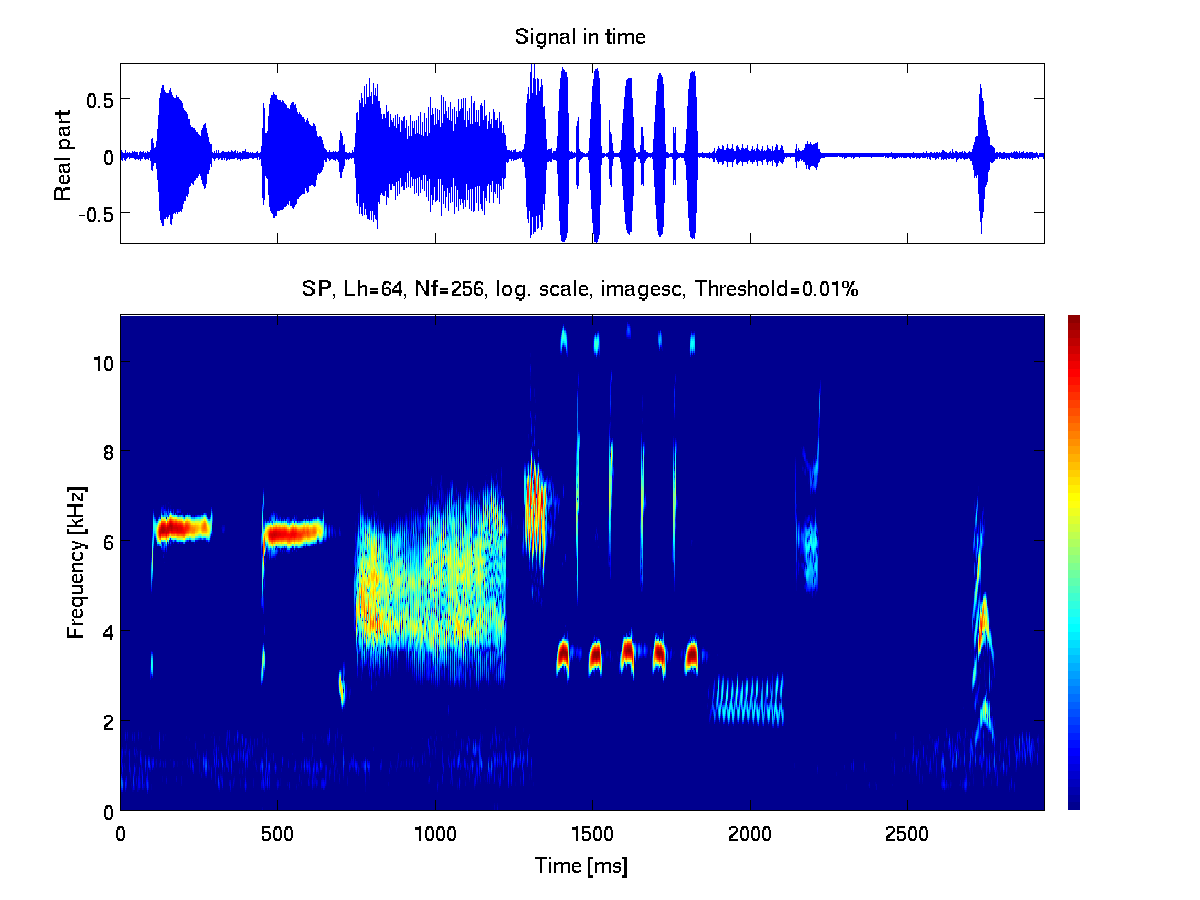
\includegraphics[width = 0.75\textwidth]{fig/example_tfd.png}
\caption{Example of time frequency distribution (TFD) \cite{TFTB-38:online}}
\label{fig:example_tfd}
\end{figure}

\section{Methodology}
\subsection{Theory of STFT}
STFT comes from traditional Fourier transform that utilizes a short time window to slice the signal into segments. Within the short time window, the signal can be assumed to be stationary. Afterwards, fast Fourier transform (FFT) will be performed on the windowed signals and generate time frequency energy distribution. The STFT energy distribution is calculated as:
\[ P_{STFT}(t,\omega) = { \left| \int { s(\tau  } )h(\tau -t){ e }^{ -j\omega \tau  }d\tau  \right|  }^{ 2 } \]
where $s(\tau)$ is the signal and $h(\tau -t)$ is the window function selected by the user \cite{leon1995time}.

Fig.\ref{stft_explanation} gives us a more direct illustration on the calculation procedure of STFT. There are few key concepts involved.

\begin{itemize}
\item nfft: number of points used to do FFT
\item hop size: relevant to time scale resolution. A smaller hop size gives higher time scale resolution but needs more computation
\item window size: =equal to nfft in the project. It determines the size of signal segment for performing FFT.
\item fs: sampling rate, related to the signal itself.
\end{itemize}

\begin{figure}[H]
\centering
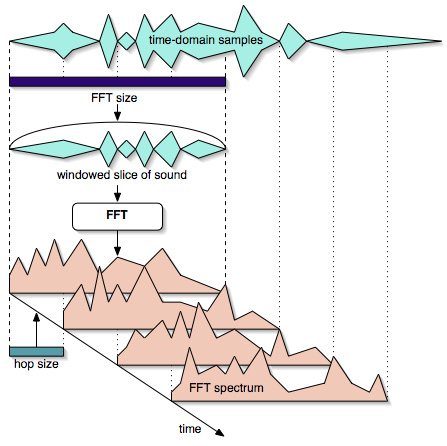
\includegraphics[width = 0.8\textwidth]{fig/stft_explanation.jpg}
\caption{Parameters for STFT \cite{ThePh65:online} }
\label{stft_explanation}
\end{figure}

\subsection{Class definition}
The program is implemented in C++. There are majorly two classes and two structs involved, as given below:

\begin{lstlisting}[language=C++]
// class for storing signals
class Signal
{
private:
	int length;
	vector<float> data;

public:
	Signal();
	Signal(int);
	~Signal();
	void ReadInSignal(const char*);		// read in signal from a text file
	void PrintSignal();					// print first and last few element of the signal
	int GetLength();						// get signal length
	float* GetSigPtr();					// get pointer to the first element
};

// struct for storing FFT parameters
struct ParaSTFT{
	int nfft;		   // number of fft points(>=wlen)
	float fs;		   // sampling frequency
	int wlen;		   // window length
	int hop;		      // hop size (<=wlen)
	ParaSTFT(){nfft=1024; fs=1000; wlen=2048; hop=512;};
};

// struct for storing parallelization parameters
struct ParaParallel{
   int nthread;      // number of thread in openMP
   ParaParallel(){nthread = 4;};
};

// class for performing STFT calculation
class STFT
{
public:
	STFT(Signal*,ParaSTFT*,ParaParallel*);
	~STFT();
	void InitTfd();                                 // initialize vector<vector<float> > tfd
   void ZeroTfd();                                 // make tfd element being 0
   //-------------------------------------------------------------------------------
   void Sequential(Signal*);                       // function for sequential calculation
	void GenLocalTfd(int, int, float*);             // generate tfd for a segment of signal   
	void PrintTfd();
   //-------------------------------------------------------------------------------
   void Parallel(Signal*);                         // function for parallel calculation
   void GenLocalTfdPar(int, int, float*);          // generate tfd for a segment of signal
   void PrintTfdPar();
   //-------------------------------------------------------------------------------
   // function for parallel calculation with MPI
   void ParallelMPI(Signal* MySignal, int idx_s, int idx_e);   
   float max_energy;                               // maximum energy in the tfd
   vector<vector<float> > tfd;                     // time frequency distribution (tfd)

private:
	ParaSTFT* para; 		                           // parameter for STFT
   ParaParallel* para_par;                         // parameter for parallelization
	int time_length;	                              // time_length
};
\end{lstlisting}

\subsection{Parallel Implementation Consideration}
In STFT, fast Fourier transform (FFT) is applied to a segment of signal (windowed signal). It provides us the opportunity to perform calculation in parallel, as suggested in Fig.\ref{stft_explanation}. To avoid repeated work, I will utilize a open-source library for performing FFT, namely "kissFFT". If faster speed is required, I would recommend using FFTW. The parallel computing will be done as follows:
\begin{itemize}
\item Process each chunk of signals in parallel (Parallel STFT calculation), as generating local spectrum P(t,f) is parallelizable. In other word, P(t=1s,f) and P(t=10s,f) can be calculated simultaneously. It should be pointed out that we will repeatedly operate on the same signal (same memory location, majorly read operation). Therefore, developing a scheme to prevent different processors going same position will largely enhance the calculation speed.

\item Generate elements of final png image in parallel (Parallel image generation). Once we have the energy distribution, we can generate a RGB image to visualize the distribution. Such repeated calculation can be parallelize and will greatly shorten program running time.
\end{itemize}

\subsubsection{Parallel STFT calculation}
Firstly, I will talk about how to process each chunk of signals in parallel. In the following code, "MySignal" is the C++ class "Signal" that stores a vector of float number (the signal), "tfd" is a 2D matrix implemented using C++ vector that stores energy in joint time and frequency space, "GenLocalTfdPar" is function for generating time frequency distribution (tfd) for a certain period of signals, which will be shown later.\\

When implementing this part, I found that the chunk-size in "schedule(guided,chunk-size)" will affect the speed of "GenLocalTfdPar". If we select a very small chunk-size, the processors might access the same signal position (memory) at the same time and limit its performance. Therefore, the chunksize is set to be wlen (window size). \\

\begin{lstlisting}[language=C++]
    // start from signal head
    int tfd_idx = 0;
    int cur_pos = 0;
    float* sig_adr = MySignal->GetSigPtr();
    // process a segment of signal of window length in parallel
    #pragma omp parallel for schedule(guided,para->wlen) num_threads(para_par->nthread) 
        for (tfd_idx=0; tfd_idx<tfd.size(); tfd_idx++)
        {
            int cur_pos = tfd_idx*para->hop;
            GenLocalTfdPar(tfd_idx, cur_pos, sig_adr);  
        }
\end{lstlisting}


The "GenLocalTfdPar" function is given as follows. Originally, I also use openMP to parallelize the for loops inside the "GenLocalTfdPar" function but it turns out to slow down my program. Therefore, I remove all the parallel for loop inside the program. One important inside the "GenLocalTfdPar" function is the "pragma omp critical". As the maximum energy in the entire distribution needs to be stored for the purpose of normalization, I will "omp critical" to prevent simultaneous change of the variable "max energy"

\begin{lstlisting}[language=C++]
    // initialize forward FFT object
    kiss_fft_cfg fwd = kiss_fft_alloc(para->nfft,0,NULL,NULL);

    vector< std::complex<float> > hann_sig(para->wlen, 0.0);

    // initialize local spectrum
    vector< std::complex<float> > ins_spectrum(para->nfft, 0.0);
    
    // Apply Hanning Window to Signal for improving frequency resolution
    if ((sig_pos+para->wlen)<time_length){
        // energy correction factor
        float corr_fact = 1.633;
        // hanning window formula: 0.5*(1-cos(2*pi*n/N)), N=L-1
        int N = para->wlen - 1;
        // apply hanning window
        // this omp parallel harms the speed
        //#pragma omp for schedule(guided)
            for (int i=0; i<para->wlen; i++)
            {
                hann_sig[i] = std::complex<float>(corr_fact*0.5*(1-cos(2*3.1415926*i/N))*sig_adr[sig_pos+i],0.0);
            }
    }

    kiss_fft(fwd,(kiss_fft_cpx*)&hann_sig[0],(kiss_fft_cpx*)& ins_spectrum[0]);

    float max_val = 0;
    // get energy distribution
    // this omp parallel harms the speed as well
    //#pragma omp parallel for schedule(guided) reduction (max: max_val) //num_threads(para_par->nthread)
        for (int k=0;k<para->nfft;k++) {
            // Calculate Energy (1/N for Fourier Transform)
            tfd[tfd_idx][k] = (ins_spectrum[k]*conj(ins_spectrum[k])).real() / float(para->nfft);  
            if(tfd[tfd_idx][k]>max_val)
            {
                max_val = tfd[tfd_idx][k];
            }
        }

    // record maximum energy in the distribution
    #pragma omp critical
    {
        if (max_val > max_energy)
        {
            max_energy = max_val;
        }
    }

    // clear garbage
    kiss_fft_free(fwd);
    hann_sig.clear();
    ins_spectrum.clear();
    kiss_fft_cleanup();
\end{lstlisting}

\subsubsection{Parallel image generation}
In this section, I use libpng++ to generate final images and a function from stack-overflow to transform gray scale image to RGB scale image, which are listed below. For parallel image generation, I use collapse(2) to combine the two for loops and use guided scheduler.

\begin{lstlisting}[language=C++]
    // plot colored image
    png::image< png::rgb_pixel > imagePar(img_height, img_width);
    // combine two for loops into one, for image generation
    #pragma omp parallel for collapse(2) schedule(guided,para_par->nthread) num_threads(para_par->nthread) shared(imagePar)
        for (size_t y = 0; y < imagePar.get_height(); ++y)
        {
           for (size_t x = 0; x < imagePar.get_width(); ++x)
           {
                if(max_energy>0){
                    // normalized intensities
                    double tmp = ((tfd[x][y])/(max_energy));
                    // transform intensity into colormap
                    COLOUR tmp_color = GetColour(tmp,0,1);
                    imagePar[y][x] = png::rgb_pixel(255*tmp_color.r, 255*tmp_color.g, 255*tmp_color.b);
                }
           }
        }
    imagePar.write("tfd_par.png");
    
//---------------- From Stackoverflow-------------------------------//
//http://stackoverflow.com/questions/7706339/grayscale-to-red-green-blue-matlab-jet-color-scale
// Transform gray scale image to RGB scale, credit to stackoverflow

typedef struct {
    double r,g,b;
} COLOUR;

// Input gray scale and give minimum and maximum
COLOUR GetColour(double v,double vmin,double vmax)
{
   COLOUR c = {1.0,1.0,1.0}; // white
   double dv;

   if (v < vmin)
      v = vmin;
   if (v > vmax)
      v = vmax;
   dv = vmax - vmin;

   if (v < (vmin + 0.25 * dv)) {
      c.r = 0;
      c.g = 4 * (v - vmin) / dv;
   } else if (v < (vmin + 0.5 * dv)) {
      c.r = 0;
      c.b = 1 + 4 * (vmin + 0.25 * dv - v) / dv;
   } else if (v < (vmin + 0.75 * dv)) {
      c.r = 4 * (v - vmin - 0.5 * dv) / dv;
      c.b = 0;
   } else {
      c.g = 1 + 4 * (vmin + 0.75 * dv - v) / dv;
      c.b = 0;
   }

   return(c);
}
\end{lstlisting}


\section{Result $\&$ Discussion}
I used a chirp signal (a signal with linearly increasing frequency) to demonstrate the speed up of parallel computing. The signal was generated using MATLAB as follows and stored in a text file. 
\begin{lstlisting}[language=Matlab]
t0 = 0;
fs = 5000;
h = 1/fs;
tf = 100;
t = t0:h:tf;
signal = chirp(t,0,tf,2000);
fileID = fopen('test_sig_chirp.txt','w');
fprintf(fileID,'%f\n',signal);
fclose(fileID);
\end{lstlisting}

In the experiments, I will test the parallel performance on the local machine. This caters for the need when the signals are short and do not require the use of server. In such situation, our signals are small (less than 10MB) and we only have a desktop computer.

\subsection{Equality between sequential and parallel implementation}
Before going into performance comparison, I would like to validate the equality between my sequential implementation and parallel implementation. In the validation step, I use STFT parameters as "nfft = 512, hop=256, wlen = 512, fs = 5000". As is shown in Fig.\ref{fig:tfd_seq} and Fig.\ref{fig:tfd_par}, the sequential and parallel implementation give the same result.

\begin{figure}[H]
\centering
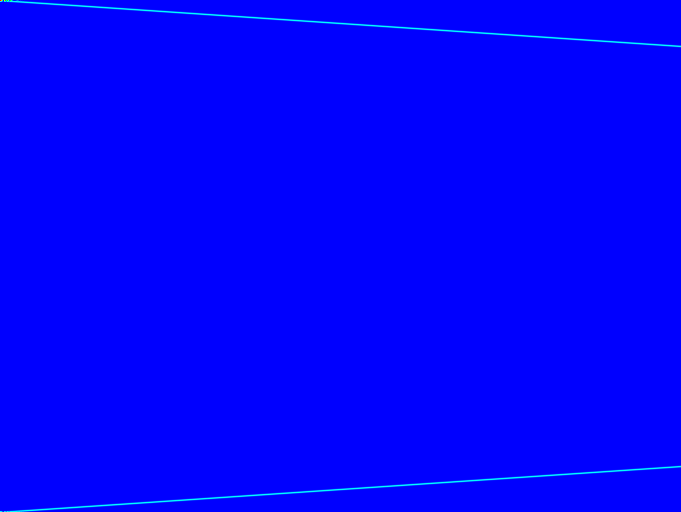
\includegraphics[width = 0.6\textwidth]{fig/tfd_seq.png}
\caption{TFD generated by Sequential Implementation}
\label{fig:tfd_seq}
\end{figure}

\begin{figure}[H]
\centering
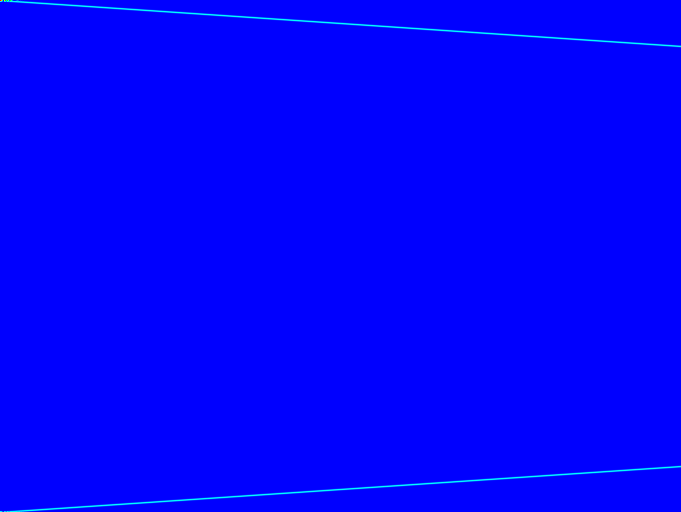
\includegraphics[width = 0.6\textwidth]{fig/tfd_par.png}
\caption{TFD generated by Parallel Implementation}
\label{fig:tfd_par}
\end{figure}

\subsection{Experiment 1: Pure openMP}

\subsubsection{Experiment Setup}
The experiment was conducted on a Dell desktop with 8 CPU and 16GB memory, with STFT parameters being "nfft = 2048, hop(hop size)=2, wlen(window size) = 2048, fs = 5000".

\subsubsection{Experiment Result}
\textbf{Number of thread}\\
As we can see, the calculation time decreases almost linearly when the number of threads increases, up to 8 threads. When it reaches 8 threads, if we keep increasing number of threads, the time will not further decrease, which is not a surprise. It is because we only have 8 CPU that limits the performance. Furthermore, although STFT calculation has almost linear speedup, the plotting process did not achieve the same speedup, which might be due to FileIO. Even though we parallelize the plotting process, the FileIO is still sequential and therefore limit the performance.

\begin{center}
  \begin{tabular}{ | l | l | l | l|  l | l |}
    \hline
    Number of Thread & STFT Time (s) & Expected Speed up & Speed up 1 & Plotting Time (s) & Speed up 2\\ \hline
    1 (sequential) & 68.180 & 1& 1 & 42.492 & 1 \\ \hline
    2 & 34.840 & 2& 1.957 & 27.264 & 1.559 \\ \hline
    4 & 17.652 & 4& 3.862 & 20.204 & 2.103 \\ \hline
    6 & 12.113 & 6& 5.629 & 17.800 & 2.387\\ \hline
    8 & 9.298 & 8& 7.333 & 16.688 & 2.546\\ \hline
    16 & 9.204 & 16& 7.408 & 16.823 & 2.526 \\ \hline
  \end{tabular}
\end{center}

\begin{figure}[H]
\centering
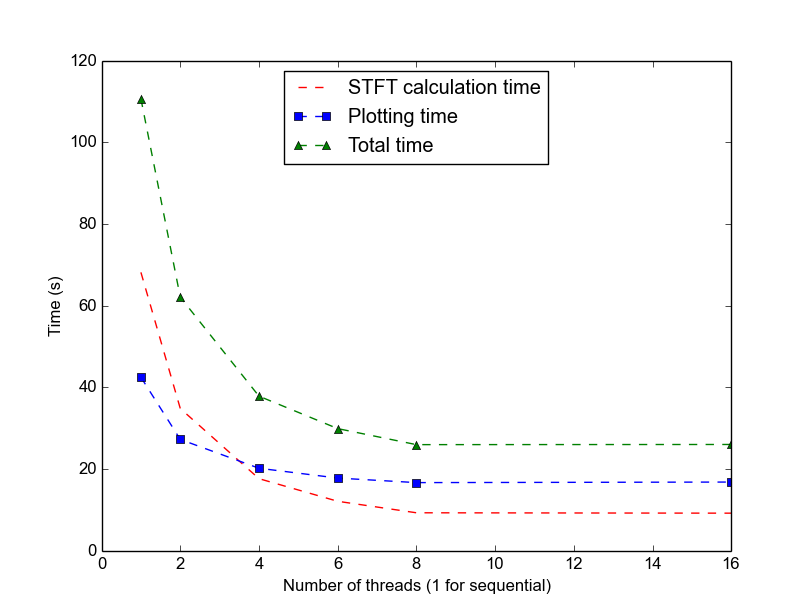
\includegraphics[width = 0.8\textwidth]{fig/local_omp.png}
\caption{Time versus number of threads}
\label{fig:local_omp}
\end{figure}

\subsection{Experiment 2: Mixed MPI and openMP Programming}
In this section, I was not able to compile the code on stampede due to the lack of library "libpng++". Therefore, I decided to develop and test the program on a local machine, as the main purpose was to play with mixed MPI and openMP programming. Here, I utilize both MPI and openMP to perform STFT calculation. This will be extremely helpful when we have a large scale audio file, enabling computation on different machines and breaking constraint of CPU limitation. As for the image generation, I just used previous code that implemented purely using openMP.

\subsubsection{Mixed Programming}
The key issues in this session is to divide jobs into different segments and apply the same function "GenLocalTfdPar" to each segments. Each node will store the whole signal but only process a certain piece of signal. Finally, the result will be gathered together. During the implementation, I found that I need to do a MPI gather to matrix type data structure. I basically follow a post on stack-overflow to implement an extended  MPI data type to cater for my need, as given below.

\begin{lstlisting}[language=C++]
	int rank, size;

	// Parameter for STFT
	ParaSTFT* para = new ParaSTFT;
	para->nfft = 1024*2;
	para->hop = 2;
	para->wlen = para->nfft;
	
	// Parallel parameter
	ParaParallel* para_par = new ParaParallel;
	para_par->nthread = 2;
	
	// Input file name and corresponding sampling frequency
	const char * fname = "../data/test_sig_chirp.txt";
	para->fs = 5000;

	//------------ MPI session ---------------------
	MPI_Status status;
	MPI_Init(&argc, &argv);
	MPI_Comm_rank(MPI_COMM_WORLD, &rank);
	MPI_Comm_size(MPI_COMM_WORLD, &size);

	Signal* data_in = new Signal();
	data_in->ReadInSignal(fname);
	
	// divide MPI jobs
	int idx_s, idx_e;
	int max_idx = floor((data_in->GetLength()-para->wlen)/para->hop);
	int seg_len = max_idx/size;

	// determine which node calculate corresponding time frequency distribution
	if(rank==size){
		idx_s = rank*seg_len;
		idx_e = max_idx;
	}
	else
	{
		idx_s = rank*seg_len;
		idx_e = (rank+1)*seg_len;
	}

//Following http://scicomp.stackexchange.com/questions/1573/is-there-an-mpi-all-gather-operation-for-matrices
	// gather tfd
	int ncols, start;
    int *allncols, *allstarts;
    MPI_Datatype columnunsized, column;

    allncols = new int[rank];
    allstarts= new int[rank];

    /* create the data type for a column of data */
    int sizes[2]    = {para->nfft, max_idx};
    int subsizes[2] = {para->nfft, 1};
    int starts[2]   = {0,0};
    MPI_Type_create_subarray (2, sizes, subsizes, starts, MPI_ORDER_C, MPI_FLOAT, &columnunsized);
    MPI_Type_create_resized (columnunsized, 0, sizeof(float), &column);
    MPI_Type_commit(&column);

	// perform STFT calculation
	double tstart_par, tend_par, elapsed_par;
	double total_elapse = 0;
	float total_max_energy = 0;

	tstart_par = omp_get_wtime();

	STFT* SigTFD = new STFT(data_in, para, para_par);
	SigTFD->ParallelMPI(data_in, idx_s, idx_e);
	
	tend_par = omp_get_wtime(); 
	elapsed_par = tend_par-tstart_par;
	

	MPI_Reduce(&SigTFD->max_energy, &total_max_energy, 1, MPI_FLOAT, MPI_MAX, 0, MPI_COMM_WORLD);
	MPI_Reduce(&elapsed_par, &total_elapse, 1, MPI_DOUBLE, MPI_SUM, 0, MPI_COMM_WORLD);
    MPI_Allgather(&(SigTFD->tfd[0][idx_s]), idx_e-idx_s, column, &(SigTFD->tfd[0][idx_s]), idx_e-idx_s,column, MPI_COMM_WORLD);

	if(rank==0){
		printf("Parallel Algorithm Calculation (MPI) Takes %6.3f seconds on average\n", total_elapse/size);
		SigTFD->PrintTfdPar();
		printf("reduced maximum energy: %f\n", total_max_energy);
	}

	MPI_Finalize();
\end{lstlisting}


\subsubsection{Experiment Setup}
The experiment was conducted on a Dell desktop with 8 CPU and 16GB memory, with STFT parameters being "nfft = 2048, hop=2, wlen = 2048, fs = 5000". For comparison purpose, I use a thread number of 2.

\subsubsection{Experiment Result}
Again, the number of CPU limits general performance. However, the speed up was less than openMP when the expected speed up is 8. It might be due to the overhead from MPI communication.

\begin{center}
  \begin{tabular}{ | l | l | l | l | l |}
    \hline
    Number of node in MPI & STFT Time & Expected Speed up & Speed up 1 \\ \hline
    1 (sequential) & 68.180 &1 & 1  \\ \hline
    2 & 17.955 & 4 &3.797\\ \hline
    3 & 12.115 & 6 & 5.628\\ \hline
    4 & 10.547 & 8 & 6.464\\ \hline
    5 & 10.470 & 10 & 6.512\\ \hline
    6 & 10.826 &  12 & 6.298\\ \hline
  \end{tabular}
\end{center}

\begin{figure}[H]
\centering
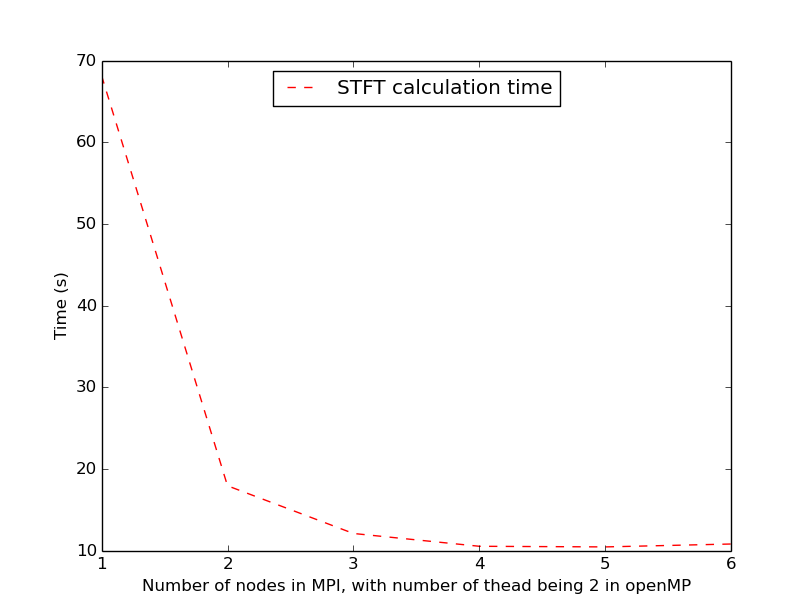
\includegraphics[width = 0.6\textwidth]{fig/local_mpi.png}
\caption{Time versus number of node in MPI (tested on local machine)}
\label{fig:local_mpi}
\end{figure}


\section{Conclusion}
In this project, a parallel version of STFT is implemented and achieve almost linear speed-up compared to sequential version of STFT. Furthermore, mixed MPI and openMP programming was explored and has achieved success. Although the parallel mechanism inside my algorithm is not that complicated, this parallel version of STFT will help my research greatly by tremendously shortening my computational time as well as providing a chance for online time-frequency analysis to biomedical signals. Therefore, I would like to express my greatest gratitude to TACC, in particular, Victor Eijkhout and Charlie Dey.

\bibliography{mycite}
\bibliographystyle{ieeetr}

\end{document}
	% line of code telling latex that your document is ending. If you leave this out, you'll get an error
